\label{chap:stand-der-technik-strassenschilderkennung}
Eine Straßenschilderkennung zählt mittlerweile zu der Standardausstattung vieler Neuwagen. Im Jahr 2024 tritt zudem eine EU-Verordnung in Kraft, durch die sämtliche neu produzierten Fahrzeuge mit einer solchen Funktion ausgestattet werden müssen \cite{eu-regulation}. Daran zeigt sich, dass das Thema bereits weitreichend etabliert ist.

Straßenschilder werden zu folgendem Zweck eingesetzt: Sie sollen Informationen über die Verkehrssituation und über geltende Vorschriften des Gebiets, in dem sich das Fahrzeug zu einem gegebenen Zeitpunkt befindet, präsentieren. Straßenschilder kommunizieren unter anderem Geschwindigkeitsvorgaben, Gefahrenhinweise und allgemeine Verkehrsregeln. Dabei sind die Schilder so konzipiert, dass sie sich visuell möglichst von ihrem Hintergrund abheben und leicht voneinander zu unterscheiden sind. Automatische Straßenschilderkennungen können Fahrzeugführende in Situationen unterstützen, in denen sie Schilder übersehen oder gezielt missachten. Anstelle dass ein reales Schild beispielsweise nur für einige Sekunden sichtbar ist, bevor es außerhalb der Sichtweite des Fahrzeugführenden ist, ist eine durchgehende Anzeige auf den Displays eines Fahrzeugs möglich. Auch akustische Warnungen oder ein aktives Eingreifen von Sicherheitssystemen sind denkbar, beziehungsweise bereits in Serienfahrzeugen vorhanden. \cite{traffic-sign-detection-review-2014}

Eine Straßenschilderkennung erfolgt visuell und wird somit mittels Kameras umgesetzt. Dabei lassen sich viele Schilder durch eine bestimmte Form (Kreis, Dreieck, Achteck, etc.) und ein Symbol (Schneeflocke, Person, etc.) oder eine Zahl identifizieren. Somit existieren verschiedene Arten von Straßenschildern, die durch den Erkennungsalgorithmus identifiziert werden. Die praktische Umsetzung solcher Algorithmen verwendet häufig \acp{CNN}, welche in Kapitel \ref{chap:KNNs} thematisch aufgeführt sind. Besonders relevant für das Thema dieser Studienarbeit ist, wie zuverlässig die momentan ausgelieferten Straßenschilderkennungen sind und welche Situationen die Algorithmen am ehesten zu falschen Aussagen verleiten. Auf dieser Grundlagen kann sich orientiert werden, welche Arten von Bildern vermehrt generiert werden sollen, um die Straßenschilderkennung verbessern zu können. \cite{traffic-sign-detection-review-2014}

Im Jahr 2019 hat eine Automobilzeitschrift die Straßenschilderkennung von unterschiedlichen Fahrzeugherstellern getestet \cite{strassenschilderkennungTest}. Zudem existieren verschiedene Publikationen, die sich mit der Thematik befassen \cite{traffic-sign-detection-review-2014}. Die Ergebnisse des Zeitschriftenartikels weisen darauf hin, dass die Straßenschilderkennung einiger Fahrzeuge bereits weitreichend funktioniert. Die Systeme sind dazu in der Lage, Geschwindigkeitsvorgaben überwiegend zu erkennen und dem Fahrzeugführenden auf einem Display anzuzeigen. Auch existieren bereits akustische Warnungen bei einer Überschreitung der Höchstgeschwindigkeit. Dennoch gibt es einige Situationen, die bei mehreren Fahrzeugen zu Problemen bei der Straßenschilderkennung geführt haben. Eine Auswahl davon zeigt Abbildung \ref{fig:einfluesse-strscherkennung}.  \cite{strassenschilderkennungTest} 

\begin{figure}[H]
   \centering
   \captionsetup[subfigure]{labelformat=empty}
   \begin{subfigure}[b]{0.125\textwidth}
       \centering
       
\includegraphics[height=\textwidth]{../images/Schilder Beispiele/Aufhebungsschild.png}
       \caption{Aufhebung}
       \label{fig:aufhebungsschild}
   \end{subfigure}
   \hspace{3em}%
   \begin{subfigure}[b]{0.125\textwidth}
       \centering
       \includegraphics[height=\textwidth]{../images/Schilder Beispiele/Ungültig.png}
       \caption{Ungültigkeit}
       \label{fig:abgeklebt}
   \end{subfigure}
   \hspace{3em}%
   \begin{subfigure}[b]{0.125\textwidth}
       \centering
       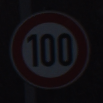
\includegraphics[height=\textwidth]{../images/Schilder Beispiele/Dunkelheit.png}
       \caption{Dunkelheit}
       \label{fig:dunkelheit}
   \end{subfigure}
   \hspace{3em}%
   \begin{subfigure}[b]{0.125\textwidth}
    \centering
    \includegraphics[height=\textwidth]{../images/Schilder Beispiele/LED.png}
    \caption{LED Schilder}
    \label{fig:ledschild}
   \end{subfigure}
      \caption{Erschwerende Einflüsse auf die Straßenschilderkennung \cite{GTSRB} \cite{led-schild}}
      \label{fig:einfluesse-strscherkennung}
\end{figure}

Fahrzeuge verschiedener Hersteller haben in den Tests Aufhebungsschilder nicht korrekt interpretiert. Damit sind Schilder gemeint, die entweder Geschwindigkeitsbegrenzungen oder Überholverbote außer Kraft setzen. Des Weiteren sorgten mittels Klebestreifen als ungültig erklärte Schilder, in einigen Fällen Dunkelheit, beispielsweise in Tunneln, und sogenannte LED \emph{Wechselverkehrszeichen} für falsche Aussagen. Auch erkennen die Systeme in einigen Situationen nicht, dass Schilder für eine kreuzende Straße gelten, statt für die Straße, auf der sich das Fahrzeug zu dem Zeitpunkt befinden. Weitere Aspekte, die in dem Artikel nicht explizit genannt sind, aber laut einer Publikation von 2014 in der Vergangenheit zu Schwierigkeiten geführt haben, sind mitunter die folgenden: \cite{traffic-sign-detection-review-2014}

\begin{figure}[H]
   \centering
   \captionsetup[subfigure]{labelformat=empty}
   \begin{subfigure}[b]{0.125\textwidth}
       \centering
       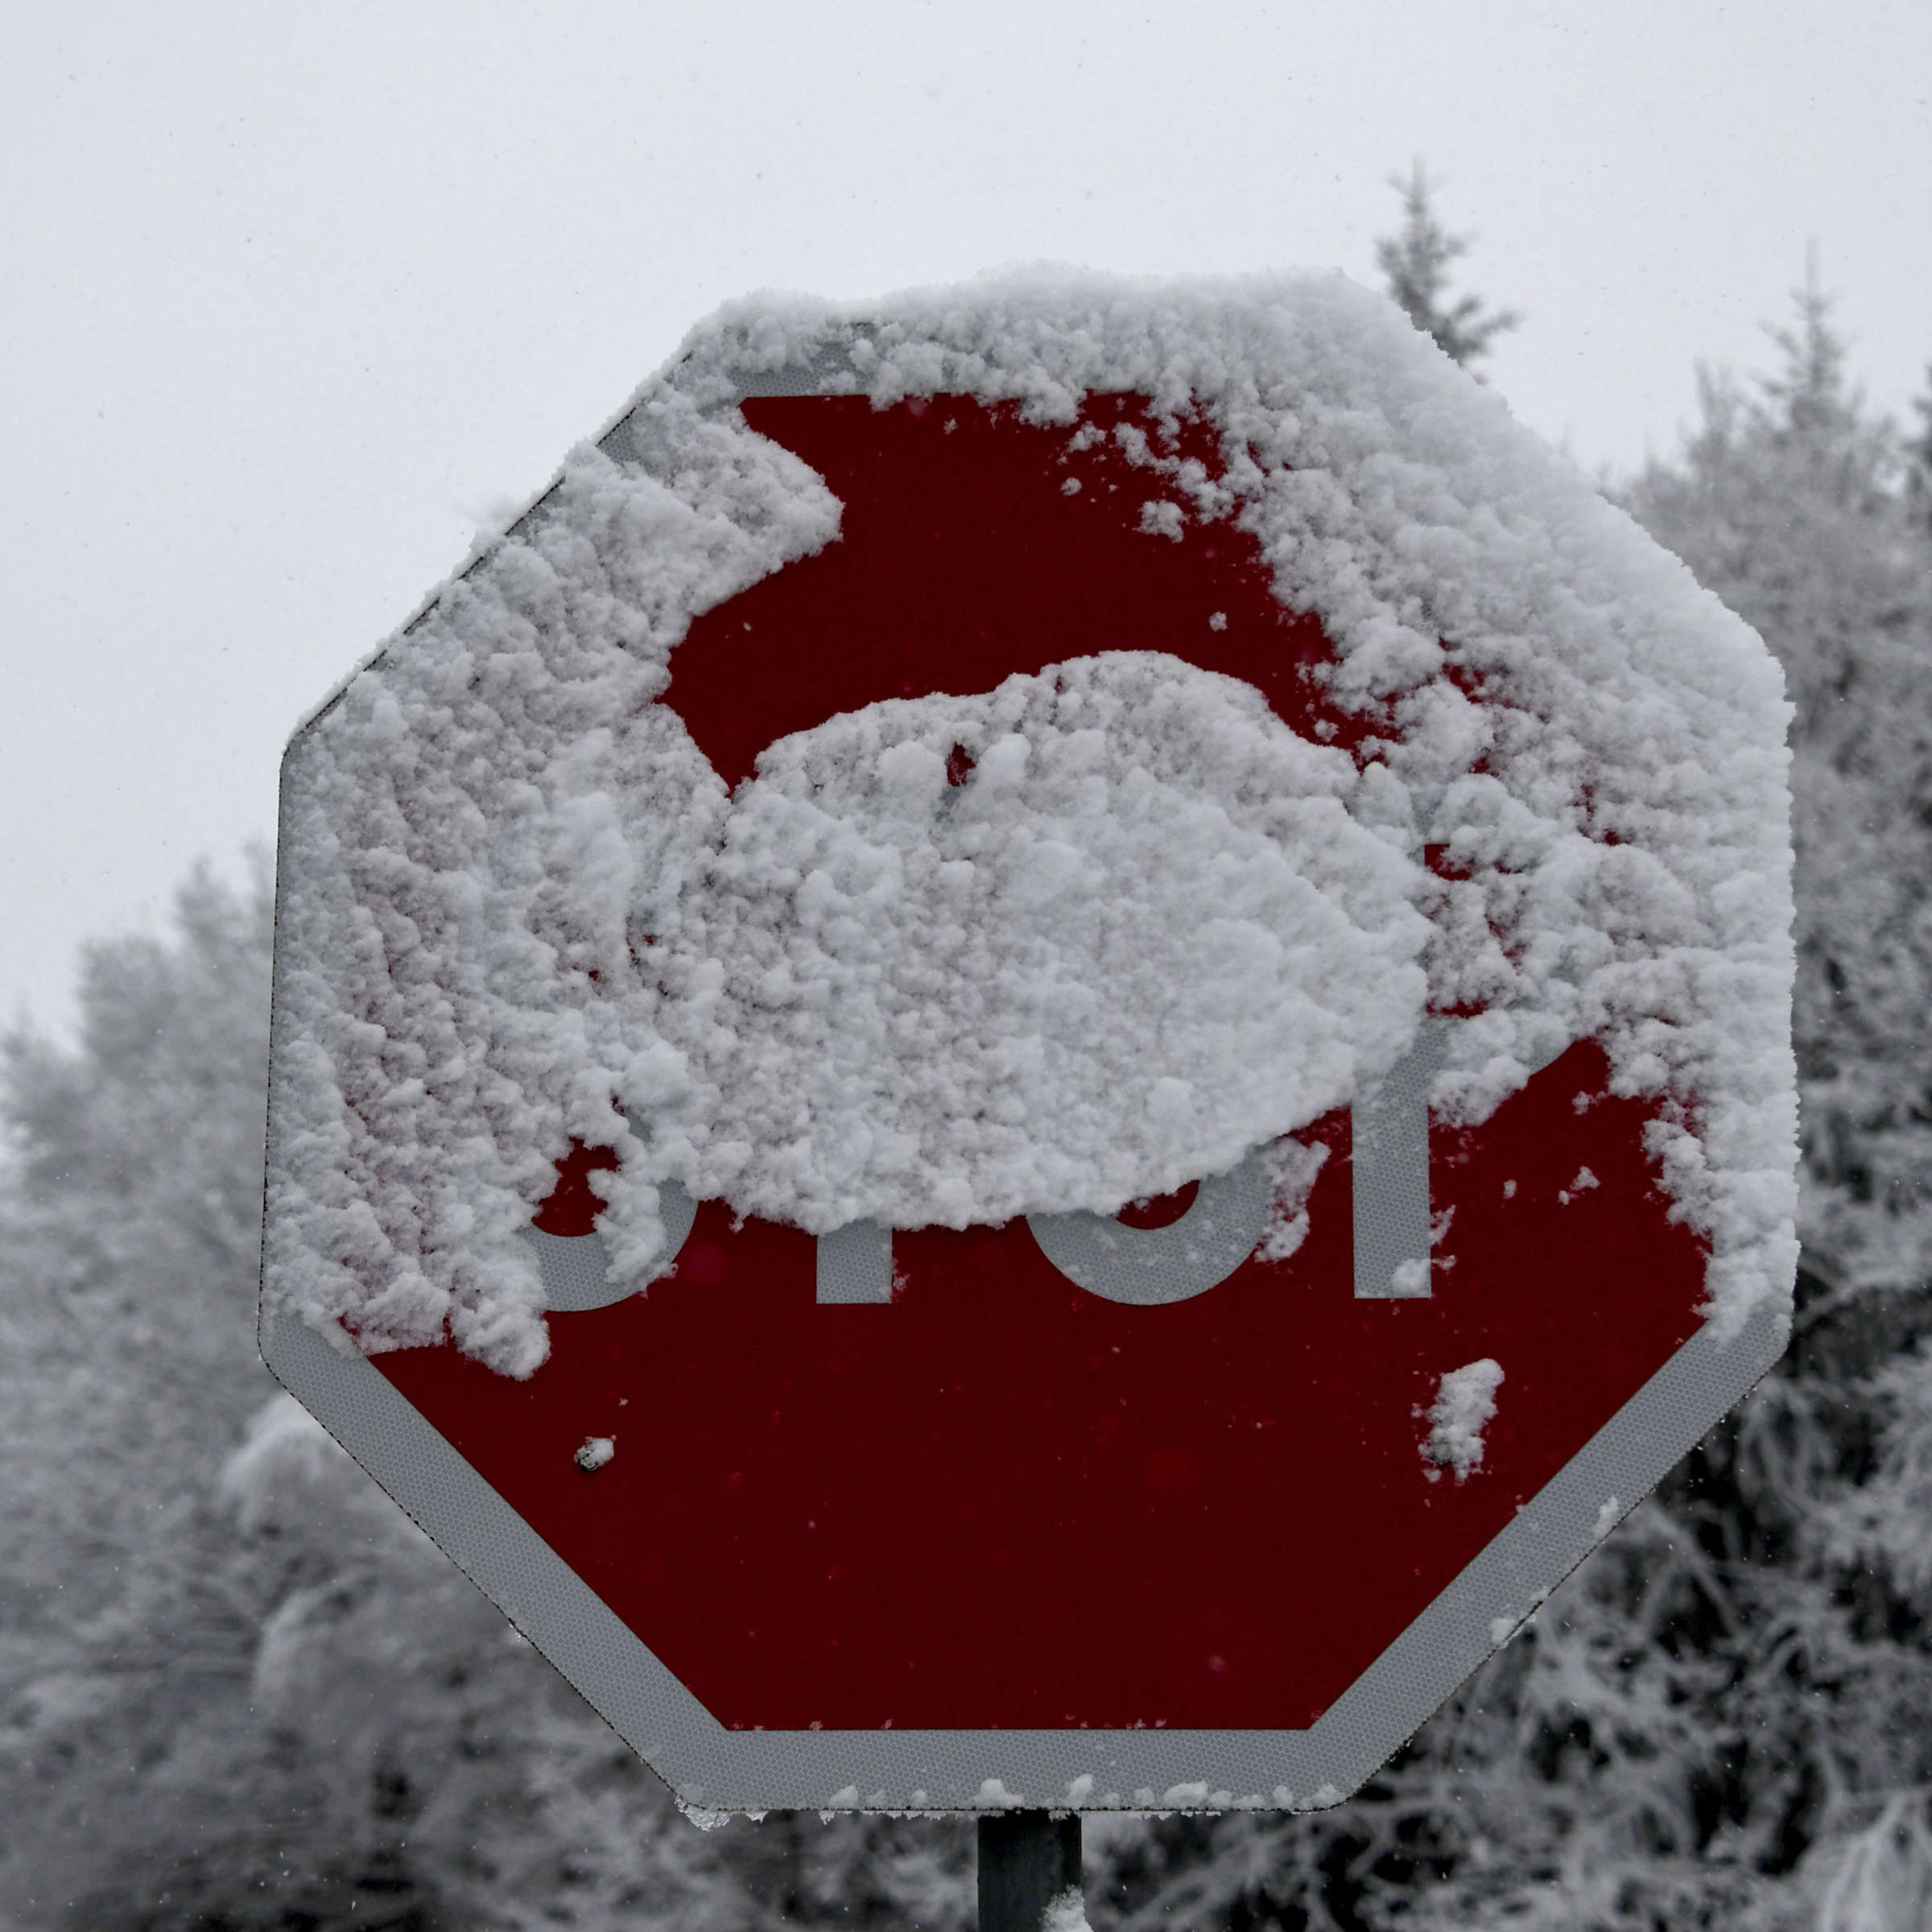
\includegraphics[height=\textwidth]{../images/Schilder Beispiele/Schnee.jpg}
       \caption{Witterung}
       \label{fig:witterung}
   \end{subfigure}
   \hspace{3em}%
   \begin{subfigure}[b]{0.125\textwidth}
       \centering
       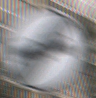
\includegraphics[height=\textwidth]{../images/Schilder Beispiele/MotionBlur.png}
       \caption{Unschärfe}
       \label{fig:motion-blur}
   \end{subfigure}
   \hspace{3em}%
   \begin{subfigure}[b]{0.125\textwidth}
       \centering
       \includegraphics[height=\textwidth]{../images/Schilder Beispiele/Überbelichtung}
       \caption{Belichtung}
       \label{fig:ueberbelichtung}
   \end{subfigure}
   \hspace{3em}%
   \begin{subfigure}[b]{0.125\textwidth}
    \centering
    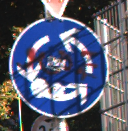
\includegraphics[height=\textwidth]{../images/Schilder Beispiele/Vandalismus.png}
    \caption{Vandalismus}
    \label{fig:vandalism}
   \end{subfigure}
      \caption{Weitere mögliche Einflüsse auf die Straßenschilderkennung \cite{GTSRB} \cite{schnee-schild}}
      \label{fig:einfluesse-strscherkennung2}
\end{figure}

Eine weitere Publikation aus dem Jahre 2019 zeigt, dass die Qualität der Straßenschilderkennung von der Stärke der äußeren Einflüsse abhängt. Vergleichsweise geringfügig verdeckte Schilder hat das Testfahrzeug hier in der Regel korrekt klassifizieren können. Sobald eine größere Fläche des Schilds verdeckt ist oder das Schild vermehrt beschmutzt ist, kann das System die Schilder zum Teil nicht mehr identifizieren. Auch hier schreiben die Autoren, dass das Wetter und somit die Sichtverhältnisse einen negativen Einfluss auf die Qualität der Erkennung zeigen. \cite{traffic-sign-anomalies}

Die Erkenntnisse der Tests aus den genannten Artikeln geben Hinweise auf das folgende: In einigen genannten Situationen können sich Fahrzeugführende nicht vollständig auf die Straßenschilderkennung ihrer Fahrzeuge verlassen. Ein Ziel der Hersteller ist das Anbieten von vollständig autonomen Fahrzeugen. Damit das möglich ist, muss die Software der Fahrzeuge auch solche Grenzfälle korrekt interpretieren. Das erfordert eine gewisse Menge an Daten, durch die diese Algorithmen trainiert werden.

Ziel dieser Arbeit ist ausgehend davon, gezielt Trainingsbilder erzeugen zu können, die einige dieser Aspekte simulieren. Es soll als alternative Möglichkeit dazu vorgeschlagen werden, sämtliche Trainingsdaten für Grenzfälle eigenständig in realen Fahrsituationen aufzunehmen.

%Diese EU-Verordnung verfolgt im wesentlichen das Ziel, verschiedene sicherheitsrelevante Systeme verpflichtend %einzuführen. Dazu zählen zudem Notbremsassistenten, Müdigkeitswarner und Notbremslichter. Die %Straßenschilderkennung trägt dazu im wesentlichen durch die Möglichkeit einer Warnung bei überhöhter %Geschwindgkeit oder einer automatischen Geschwindigkeitsanpassung bei.